\chapter{Design}
The focus of this paper is to explore the differences between a single model and a multistage architecture for throughput prediction in wireless networks. The choice of machine learning or deep learning model must therefore be consistent across all models considered to avoid confusing the issue with that of comparing one ML (machine learning) or DL (deep learning) method of regression with another. Lstm (long short-term memory) networks are recognised as effective models for time series forecasting \cite{8614252}, with deep learning models in general performing well in networking related tasks \cite{8666641}. As such any individual model considered in this paper is some form of Lstm deep network. Initial comparisons of multistage vs a single model ensure that all Lstm models have the same hyperparameters. That is to say, all models have the same number of nodes, layers, the same dropout chance, activation function, optimizer, etc. The only difference between the individual models considered will be that the classifier model has a different output layer to the traditional regression models as it aims to predict the class of the input sequence as opposed to the DL\_bitrate horizon. In total there are 5 individual Lstm models that had to be trained with brief description given in \ref{tab:brief_models}

\begin{table}[!htb]
  \centering
  \caption{Lstm Deep Models Used}
  \begin{tabular}{|c|c|c|}
  \hline
    {Model} & {Training Data} & {Outputs} \\
    \hline
	Baseline & All TP examples & DL\_bitrate prediction horizon \\
	\hline
	Low & Only Low TP examples & DL\_bitrate prediction horizon \\
	\hline
	Medium & Only Medium TP examples & DL\_bitrate prediction horizon \\
	\hline
	High & Only High TP examples & DL\_bitrate prediction horizon \\
	\hline
	Classifier & All labelled TP examples & Class probability table \\
  \hline
  \end{tabular}
  \label{tab:brief_models}
\end{table}


In \ref{CONSTRAINTS HEREHERHEHREHR} the number of parameters of the Lstm models were altered in various ways in order to achieve memory size parity between the single baseline throughput predictor and the multistage predictors. This is an important point to explore as adoption of a multistage approach vs a single model on mobile devices will require that both methods have comparable performance on hardware. A multistage approach could only be considered more optimal if the required memory and inference time were comparable. By design a multistage approach will be bigger than a single model, as such the total number of parameters of both approaches should be equalised for further comparison.

\section{Model Tuning}
\label{sec:model_tuning}



\section{Baseline}
The baseline model was trained on the entire training dataset regardless of class.

\section{Multistage One}
\begin{figure}[h]
\centering
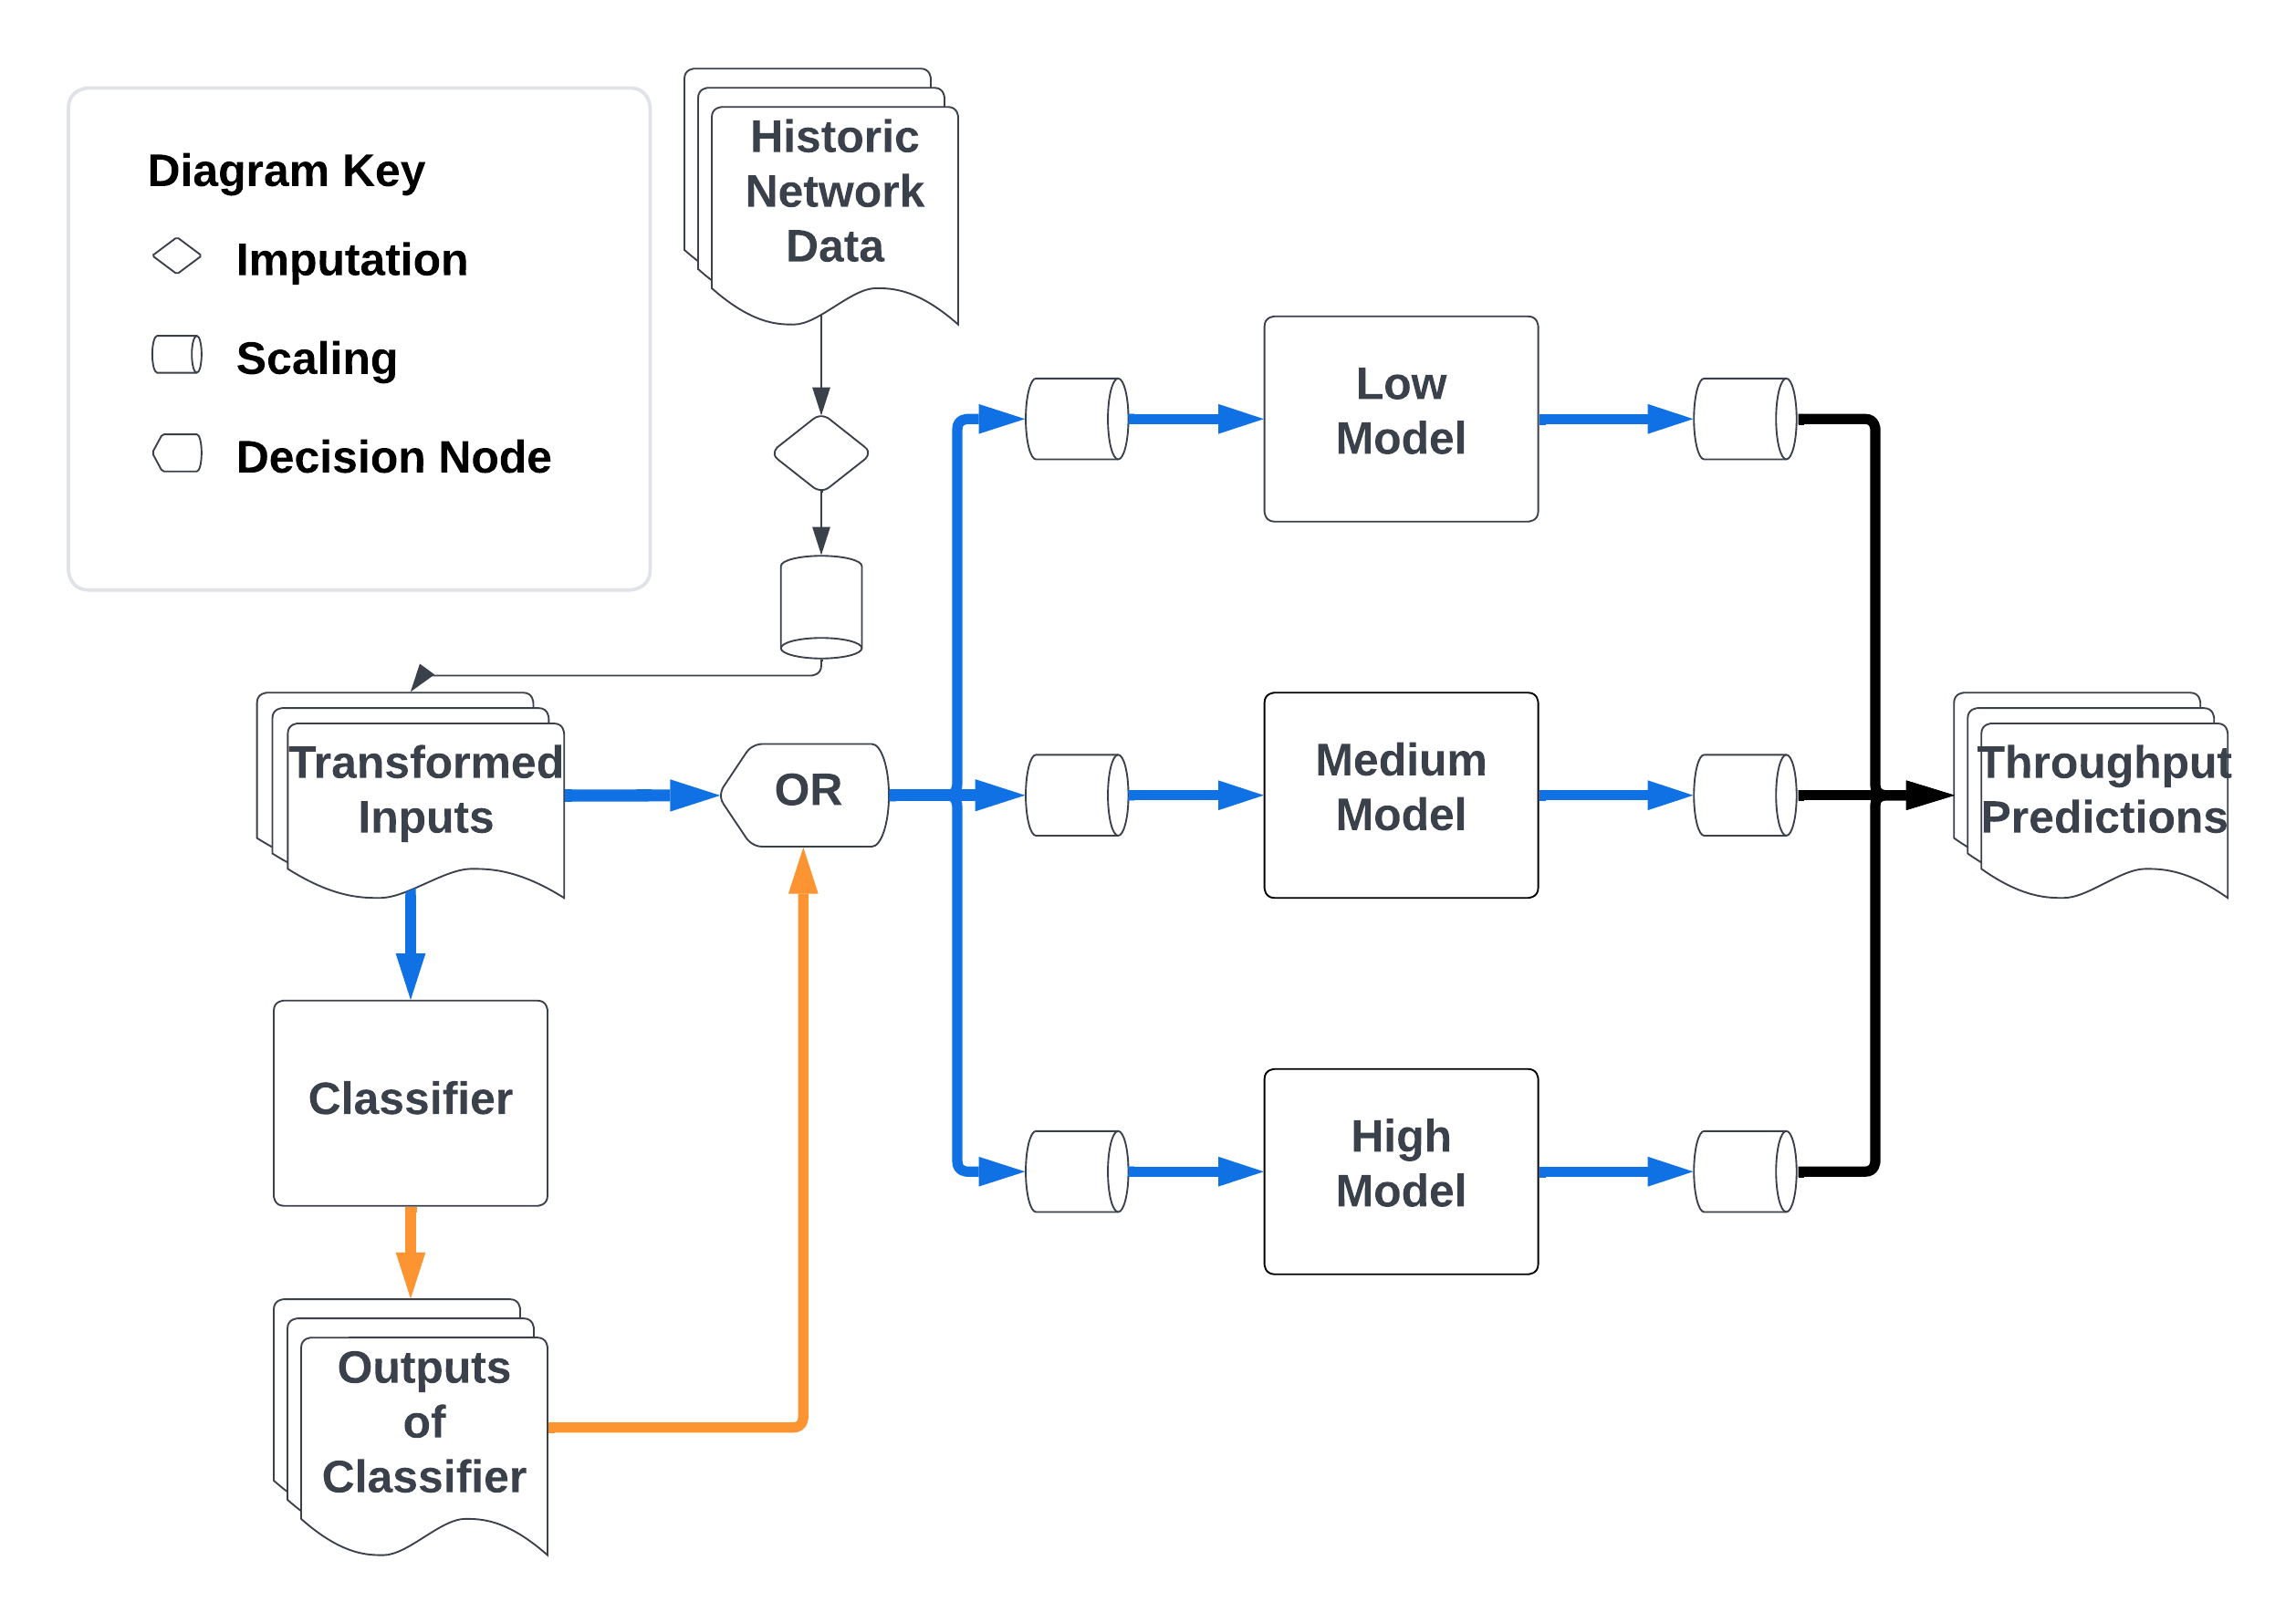
\includegraphics[scale=0.15]{Multistage One.png}
\label{fig:multistage_one}
\caption{Figure shows the structure of the Multistage One model.}
\end{figure}

The multistage throughput predictor herein referred to by "multistage one" uses a classifier to predict the most likely throughput class of the horizon for a given history sequence. As previously discussed, three classes are considered, high, medium and low, which describe the group the horizon throughput based on sub-ranges. Refer back to section \ref{sec:bounds} for a detailed description on the construction of these classes from the dataset. Based on the classifier's decision, the input is passed to one of the three regression models, each trained exclusively on examples of sequences of their respective class. As only one model is chosen, performance of this architecture is heavily dependent on correct classification of the horizon throughput scenario by the classifier. Misclassification of an input sequence will lead to the wrong regression model being chosen for throughput prediction negating the advantage of the multistage approach vs a single model entirely.

\section{Multistage All}
\begin{figure}[h]
\centering
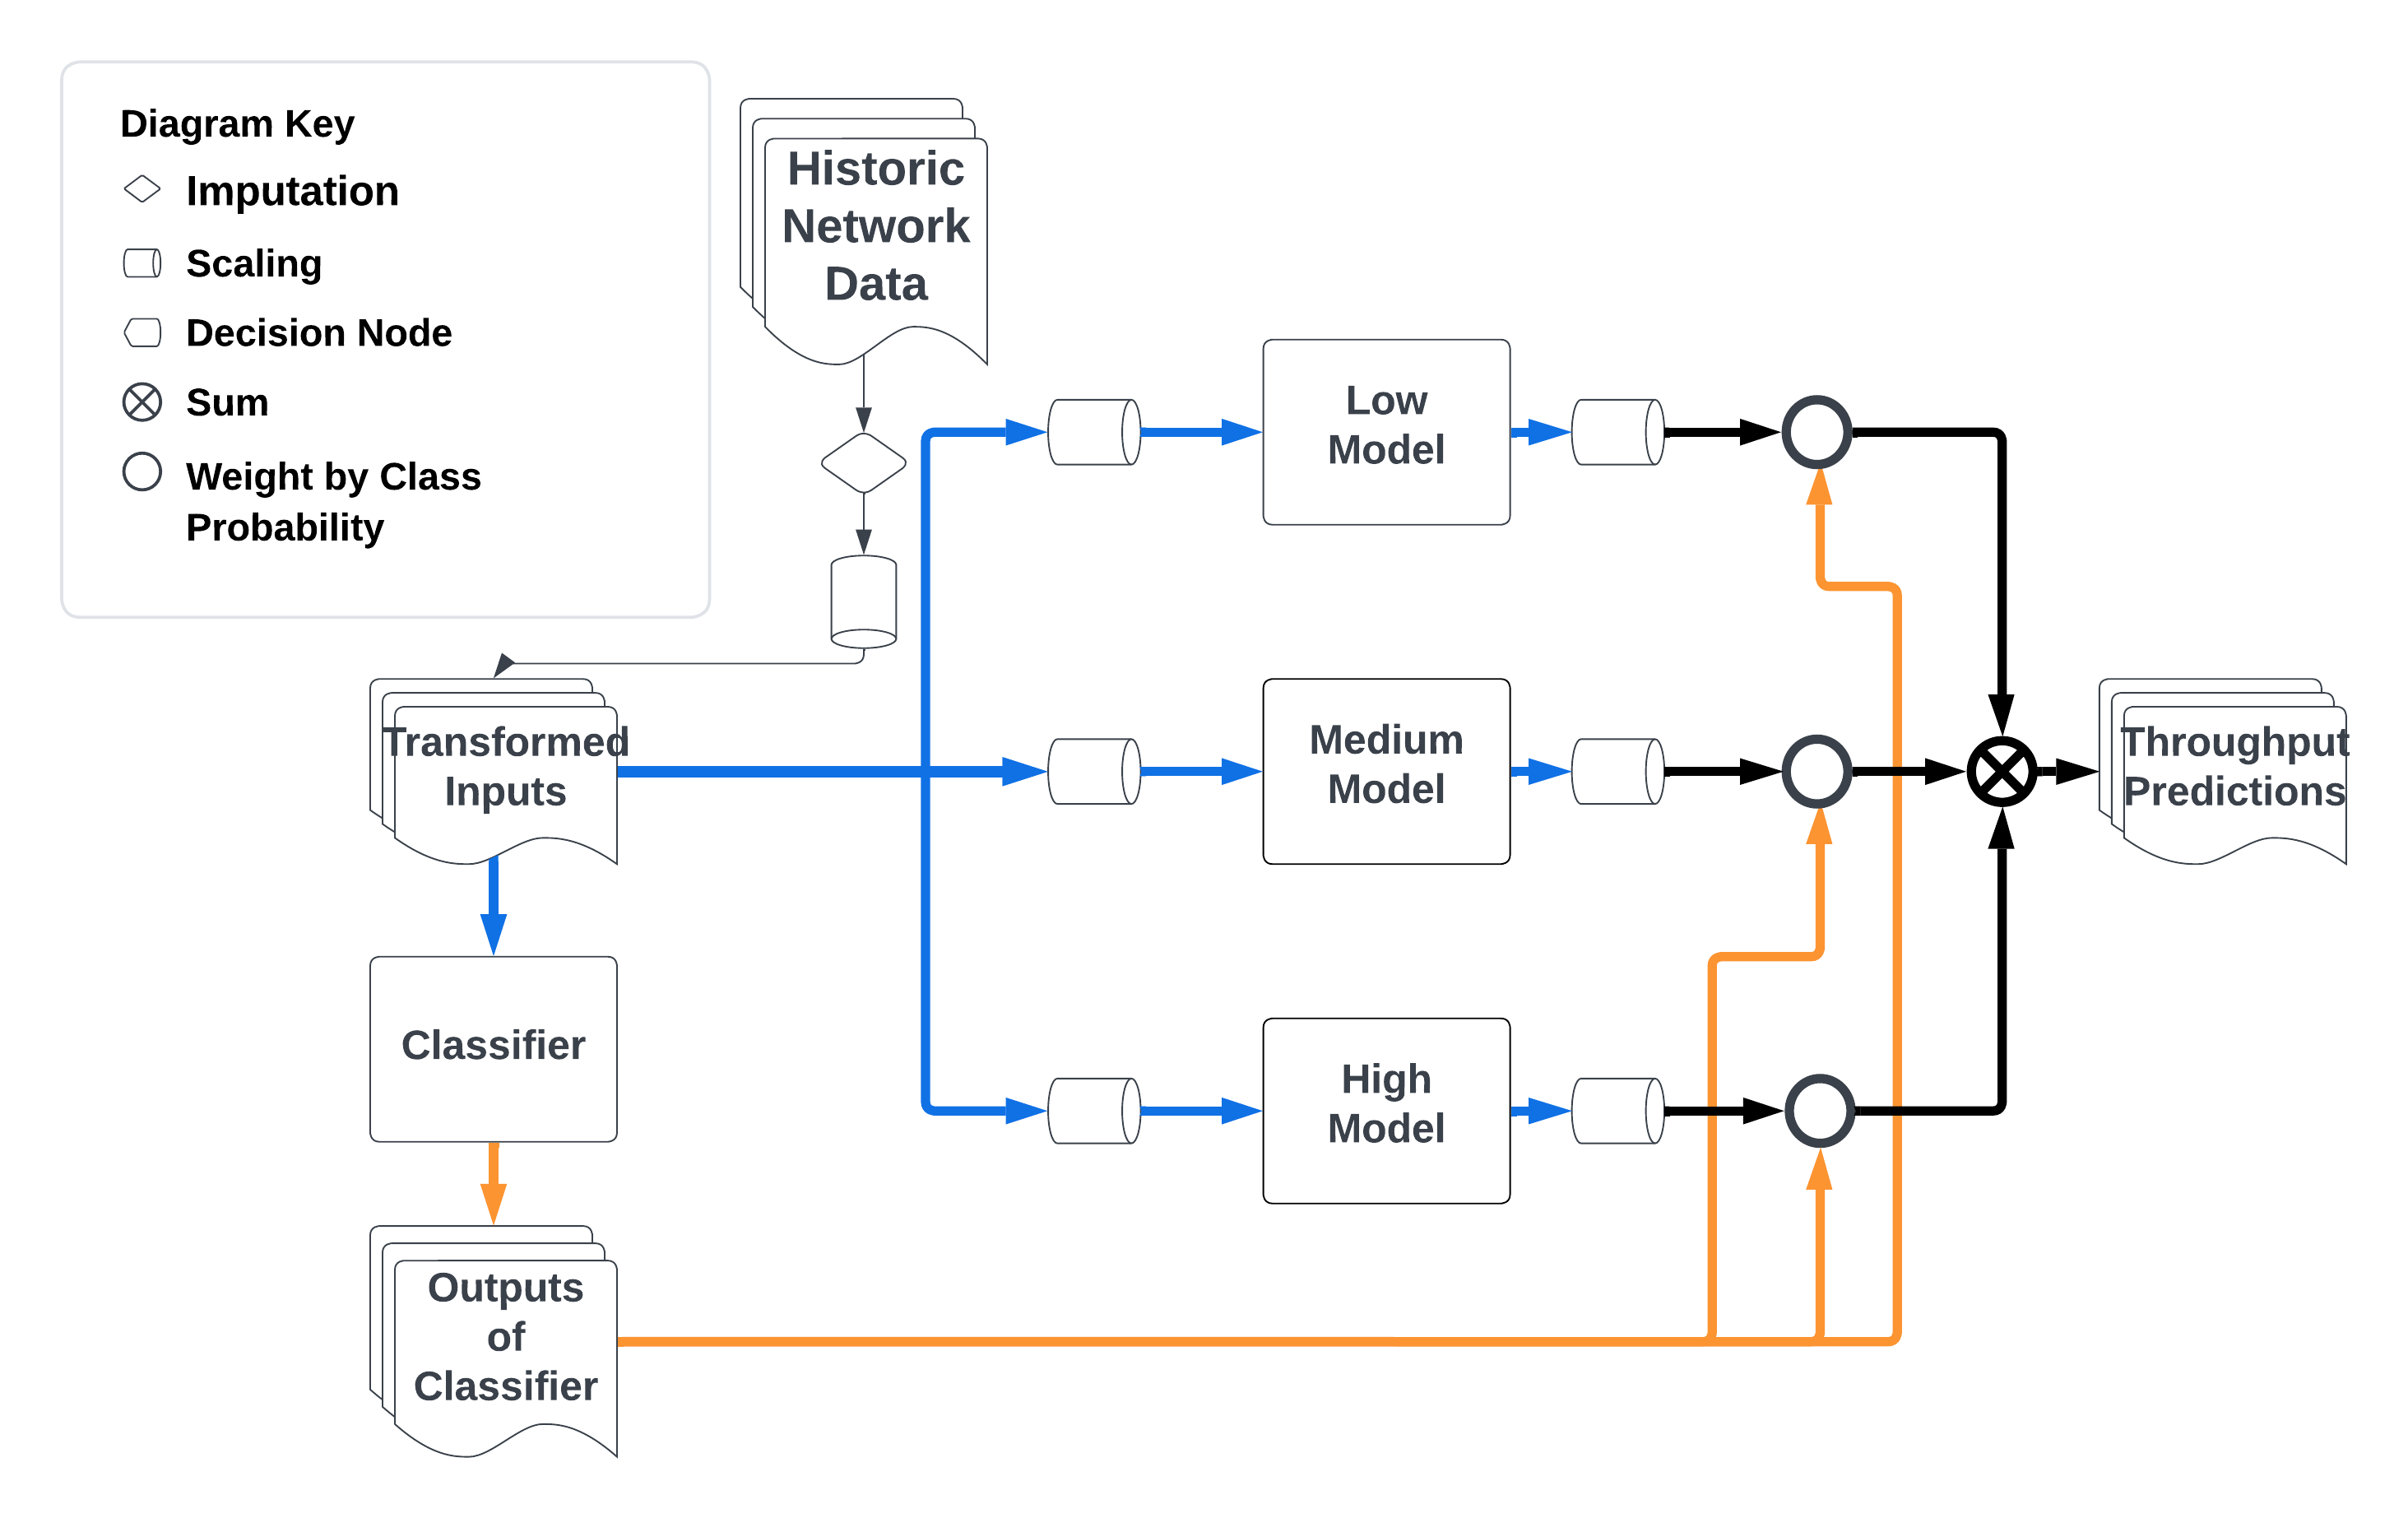
\includegraphics[scale=0.15]{Multistage All.png}
\label{fig:multistage_one}
\caption{Figure shows the structure of the Multistage All model.}
\end{figure}

The multistage throughput predictor herein referred to by "multistage all" uses a classifier to predict the probability of each of the classes of the horizon for a given history sequence. Unlike the multistage one model, the input sequence is then passed to all three regression model. The outputs of the regression models are then weighted by the class probability vector from the classifier and summed to create the final prediction. This is essentially an ensemble model. Ensemble models are known to perform better than using a single model \cite{https://doi.org/10.1002/widm.1249}. This model should perform better in situations where the classifier made less definite predictions on the input sequence's class. In theory, sequences on the border of two classes are better accommodated for by this model compared to the multistage one model.

\section{Testing Framework}